% !TeX spellcheck = en_US
\documentclass[11pt, fleqn]{article}

\usepackage{../SpeedyGonzales}
\usepackage{../MediocreMike}

\usepackage{lipsum}
\usepackage{booktabs}
\usepackage{subcaption}


\usepackage{program}
\NumberProgramstrue

\makeatletter
\def\BState{\State\hskip-\ALG@thistlm}
\makeatother 


\usepackage{xcolor}
\usepackage[normalem]{ulem}
\useunder{\uline}{\ulined}{}%
\DeclareUrlCommand{\bulurl}{\def\UrlFont{\ttfamily\color{blue}\ulined}}
\newcommand{\code}[1]{{\texttt{\footnotesize#1}}}
\newcommand{\argmin}{\ensuremath{\text{argmin}}}
\usepackage[margin=1cm]{caption}
\geometry{top=1cm}

\title{\vspace{-2cm}Playing 2048 with Policy Gradients: Deep Reinforcement Learning on a Game with Random Elements}
\author{Oskar Eiler Wiese Christensen, Søren Winkel Holm, and Asger Laurits Schultz}
\date{\today}

\pagestyle{plain}
\fancyhf{}
\rfoot{Page \thepage{} of \pageref{LastPage}}

\graphicspath{{Billeder/}}

\begin{document}
	
\maketitle
%\thispagestyle{fancy}
%\tableofcontents
\vspace*{-1cm}
\begin{abstract}\noindent
A Deep Reinforcement Learning method easily applicable to randomized problems could be generalized to solving challenging real world problems with changing environments such as autonomous vehicles and financial strategies. Games with random elements can be used as test environments for such AI, but are often solved using specialized heuristics that are not generally applicable. In this paper, we apply vanilla Policy Gradients on the game 2048, examining both different network complexities and a number of reward functions with differing degrees of specialization to find the optimal Deep Reinforcement Learning approach for such a problem. We observe that all agents improve and do outperform randomness but are far behind human ability, and that complex networks and specialized reward functions do not improve results. Conclusively, we highlight the poor robustness of Policy Gradients as a barrier for training on randomized tasks and call for testing of more cautious approaches such as Trust Region Policy Optimization and for a more systematic hyper-parameter search.
\end{abstract}

\section{Introduction}
%The purpose of this section is to introduce the reader to the topic and provide the necessary overview.
%• Why was the study undertaken?
Reinforcement learning (RL) is the subfield of machine learning concerned with training agents to perform tasks by learning from their environment and a reward signal. RL has shown large potential in areas such as optimal control and in board games like go and ATARI video games.

This study was undertaken to examine a policy-based deep learning approach to a game with significant random elements. Using a video game allows the environment to be  completely controlled  with the only limiting factor being computational power. We chose the game 2048 (playable at \url{play2048.co}), created by Gabriele Cirulli in 2014. 2048 is about combining tiles of the same value by moving them in one of four directions on a board with a new tile spawning randomly every turn.

In the experiment, several agents are trained using policy gradients (PG) with varying network complexities and reward policies, and then held up against each other. We examine whether learning is possible in this randomized environment, if more complex networks and heuristic rewards achieve better results, and whether the agents can achieve superhuman results.

Due to the simple rules and the limited observation and action space, we hypothesize that our agents are able to achieve superhuman or human performance given enough training, and that complex networks and tailored reward functions further boost the agents' performance.
\section{Methods}
\textit{Python source code available at} \url{https://lab.compute.dtu.dk/s183911/alpha2048}\\
The experiment consists of training and evaluating eight different models using two different network complexities and four different reward functions.
\paragraph{Observation Space and Action Space}
In 2048, the observation space would normally consist of all values on the board with empty tiles represented by 0. This would mean 16 input neurons in a policy network; however, we applied a one hot feature transformation. The issue with using 16 input neurons was the fact that a board position  activates the same neuron, regardless of the tile's value. In the game, there could be major differences between optimal moves depending on which tile, ie. 2 or 4, is in a certain position and the binary transformation expresses this fact more clearly. Each tile on the board can assume 16 different values, which resulted in $ 16\cdot 16=256 $ binary input neurons after the feature transformation.

The action space consists of the four possible directions: left, up, right, down.
\paragraph*{The Policy Network}
Inspired by PyTorch's tutorial \cite{Torch}, PyTorch's Neural Net module was used to create the policy network for this experiment. To examine the optimal network architecture, two policy networks with different complexities were used. Both had input layers of 256 neurons, output layers of 4 neurons, and were fully-connected networks. The simple network had a single hidden layer of 16 neurons. The complex network had two hidden layers of size 100 and 50. For non-linearity after the hidden layers in both policy networks, we applied the ReLU activation function to ensure negative values were set to 0 to improve expressiveness, and for regularization, a dropout layer with a dropout of 0.6 was used to prevent overfitting \cite{Sri}. Before the output layers, the softmax activation function was used which maps the output values to an interval [0; 1] such that the values sum to one. 
\paragraph*{Policy Update with Gradients}
When the agent chose an action in the game, it received a reward based on a reward function. In order to enhance the performance of the algorithm, the parameters of the neural network were continually updated. A gradient-based approach was used by back-propagating. The chosen action and the corresponding reward were saved after each move. At back-propagation, the output gradients were all set to 0 except for the chosen action which is set to the product of the received reward and the logarithm of its output value. Thus, a gradient was computed, and the network parameters were optimized using stochastic gradient descent (SGD) which saves computational power by only computing the gradient for a randomly sampled subset of data points. The learning rate was set to $\alpha=0.001$ based on pilot experiments. The calculation of gradients was done using the PyTorch autograd module. 
\paragraph*{Reward Functions} A reward function $R(s)$ returns a reward based on the game state $s$.  Four different functions were tested:
\begin{itemize}
	\item \textit{Score}: Simply rewarding the agent the increase in game score each turn.
	\item \textit{Variance}: A self made function that rewards the agent for compacting larger tiles as close as possible to the corner of the board. The negative variance is returned to reward a compact board.
	\item \textit{Heuristics}: A specialized 2048-function that returns reward for the degree to which each of four following strategies are used: keeping the board monotonic, e.g. the tiles in a snake-like order, having many available merges on the board, having many empty tiles and placing the biggest tile in the corner. The first and last heuristic were weighted thrice as much as the middle two.
	\item \textit{Combination}: The sum of the three previous reward functions each turn.
\end{itemize}
Further explanation of the specialized reward functions can be found in appendix \ref{reward}.

\paragraph*{Batch Learning} \textit{Also consult pseudo code at appendix \ref{pseudo}}\\
The network was trained in batches of 50 games. Moves were made by feed-forwarding the one hot representation of the game state through the network and then sampling the move using the output neurons as a probability distribution. Sampling allowed the agent to explore different strategies rather than the one which it preferred at a given state.\footnote{It should be noted that the agent was not allowed to choose actions that do not cause a change in the game state, as early experiments showed a tendency for the agent to maximize the number of moves, which was devastating for execution time, while resulting in little or no performance gain.} After each move, a corresponding reward was calculated. The reward for each state was saved in a list which, after a game, was discounted with a discount factor of $\gamma = 0.95$ such that the rewards are smoothened and late game rewards were exponentially less important \cite{Kar}. When a batch finished, rewards were standardized to have a mean of 0 and a variance of 1 by subtracting the mean and dividing by the variance. Parameter update was then performed using the rewards to back-propagate and optimize the network. 

Performing parameter updates in batches is advantageous, as it reduces the effect of non-representative games throwing learning off course. The fewer, but more costly, parameter updates are also preferable, as performing fewer, but more demanding, updates is somewhat more computationally efficient than several, less demanding, updates.
\\
\\
The two different network architectures and four different reward functions are used to construct eight different models. All other hyper-parameters were fixed with a learning rate of $\alpha = 0.001$, reward discount of $\gamma = 0.95$, dropout of 0.6 and SGD as optimizer, and the models were trained for 500 batches consisting of 50 games each.
\subsection*{Model Evaluation Protocol}
%Tilføj deterministisk - hvis vi vil ;);)););))
\paragraph{Collecting Playing Results} After training as per above training procedure, the performance of agents was evaluated. A number of batches consisting of 50 games were played by the agents and their score means were saved. The mean of these $N$  batch means is the result. A sample size $N$ of  batches was calculated based on a desired margin of error and expected standard deviation $\sigma $ using: $ N =z_{\nicefrac{\alpha}{2}}^2\left(\dfrac{\sigma}{E}\right)^2 $\ assuming normal distribution. From training experience, it was observed that for a worst case scenario, a $\sigma$ for the batch means can be approximated to $\sigma \lessapprox 200$.  A confidence level of 95\pro\ was used and a desired margin of error of $E=15$ score. The minimum sample size was calculated to 683, and a sample size of 700 batches was chosen.\\\\
The game was played by an agent by forward-passing the game board each turn and choosing an action based on the highest output-neuron activation: $|argmax|(outputlayer)$. Sampling was not done during the evaluation process, as exploration was not necessary when not in a learning setting.
\paragraph{Analysis of Results}
The score was used as the primary metric for the performance of agents. To be able to compare performance of different agents, confidence intervals of the mean score of the batch means were calculated. The mean scores appear normally distributed\footnote{This was part of the reason for choosing batch evaluation: besides giving a continuity from training, it places the data points in a normal distribution.} and the confidence interval for the mean score of 700 batches was calculated using a confidence level of 95\pro:
$
\bar{x} \pm 1.96\cdot  \frac{\sigma}{\sqrt {700}}
$
 

%This section should describe the experiment in full detail, such that it would be possible for the reader to reproduce
%it. This section should be written in past tense.
%• When, where, and how was the study done?
%• What materials and software was used?


%• How was the experiment designed?

%• What was the experimental procedure?
%• Which methods were used to analyze the results?

\section{Results}
The distributions of maximum tiles for each agent can be found in appendix \ref{mtile}.
Histograms of scores and batchwise score means can be found in appendix \ref{hist}.
\subsection*{Learning Processes of Agents}

See plots of all learning processes in appendix \ref{plotlearn}. Two learning processes deemed representative are shown here:
\begin{figure*}[h!]
	\centering
	\begin{subfigure}[t]{0.4\linewidth}
		\centering
		\captionsetup{width=.8\textwidth}
		\includegraphics[width = \textwidth]{"clean_train_score_complex"}
		\caption{Agent with complex policy network and score as reward}
	\end{subfigure}%
	~ \hspace{1cm}
	\begin{subfigure}[t]{0.4\linewidth}
		\centering
		\captionsetup{width=.8\textwidth}
		\includegraphics[width = \linewidth]{"clean_train_combination_complex"}
		\caption{Agent with complex policy network and combination as reward}
	\end{subfigure}
\end{figure*}

\subsection*{Agent Evaluation Scores}
\begin{table}[H]
	\centering
	\begin{tabular}{@{}l|lllll@{}}
		\toprule
		Layers / Reward& Score & Variance & Heuristics & Combination  \\ \midrule 
		256, 16, 4       &   $2335\pm 13$    & $2226\pm 11$       & $2155 \pm 12$ & $2157\pm 12$                                                                                        \\
		256, 100, 50, 4 &  $2291 \pm 12$    &          $1473 \pm 9$&            $2248 \pm 12$ &                                             $2319 \pm 13$                 \\ \bottomrule
	\end{tabular}
\caption*{Mean and 95\pro-confidence interval of mean scores in 700 batches consisting of 50 games each.}
\end{table}\noindent
Random Agent: $1094 \pm 5$
%This section should report and summarize the data that was collected and the statistical analyses that were performed.
%This section should be written in past tense.
%• What did the study find?
\paragraph{Findings}
The mean scores were not on human level. Human records\footnote{An example of a record of $1.33\ctp5$: \url{https://www.youtube.com/watch?v=YWDZqtNtdGk}} are $\gtrapprox 10^5$, and we can ourselves achieve $\sim10^4$ consistently without much difficulty.

Learning was noticeable, and most agents outperform random by $\sim 100 \pro$. The specialized reward functions were for the most part less effective than pure score reward.

Complex networks generally did not show better results and achieved in one case significantly worse score than the simple model.
%• What answer was found to the research questions?

%• Did you find evidence to confirm your hypotheses?

%The goal is to present the results without any subjective interpretation.
\section{Discussion}
\paragraph*{Learning Difficulties}
It is worth noting that simple networks rewarded by heuristics and combination functions do not indicate learning during training (see appendix \ref{plotlearn}), but, when evaluated, perform comparably to the remaining agents, clearly showing learning did happen. This could partially be explained by reward functions not correlated with score or sampling from the output layer playing an important role in performance.

Apart from that, the learning process is quite similar for all agents. Generally, the policy network improves quickly but reaches a plateau fast and does not improve any further. All agents find local optima and do not improve from that point on; in some cases even regressing in score. By observing the agents play in a UI\footnote{Animation of the simple policy network with score as reward playing: \url{https://bit.ly/2MnipEO}}, it seems that most agents find a strategy of keeping the highest tile in the corner and the two next-highest tiles in the two neighboring positions and so forth\footnote{Visualization of what the agents seem to be pursuing: \url{https://bit.ly/2sEVQ5j}}. This is a somewhat intelligent strategy, but it lacks potential for improvement.
 
Pilot experiments with different learning rates and other hyperparameters showed similar results, but a systematic hyper parameter search and tests of adaptive learning rates are needed before this learning problem can be classified as an inherent PG problem.

Apart from the stochastic elements of the game, the difficulties might stem from the continuous nature of the task yielding score for most moves, making it difficult to discern intelligence from random approaches.
\paragraph*{Optimal Networks and Parameters}
Agents generally show similar learning patterns, even though the rewards are vastly different. The comparably strong results of the pure score reward shows that PG enables the agent to discover strategies naturally as well as being explicitly rewarded for following them. As the models quickly reach local optima, there is not much benefit in the more complex networks. They generally perform similarly to the simple models, except in the case of the variance as reward which possibly is due to this self made reward function not being correlated with score.
%\subsection*{Comparisons}
\paragraph*{Other implentations of Deep Reinforcement Learning}
The most similar implementation of a vanilla policy-based network reached comparable results\footnote{Scores were not shown; they reached 1024 "a significant number of times" \cite[3.4]{Amar}. Our max. tile statistics are in \ref{mtile}}\cite{Amar}. A version using finely tuned heuristics as reward was able to push mean scores to 5600  \cite{Nie} though we could not replicate this with similar heuristics. Convolutional Q-networks seemed to outdo these; one network reaching $\sim 1.6\ctp4$ \cite{Vir}, while a similar convolutional network "did not perform well" \cite[introduction, slide 15]{Wie}. This highlights the established problem in deep reinforcement learning of reproducing results due to small differences in initialization, optimization and backpropagation methods leading to vastly different learning processes \cite{Hend}. 

\paragraph*{Non-learning Algorithms}
Some very strong algorithms have been created using heuristics and deep expectimax tree search. One example, which might be the best 2048 AI, has a median score of $1.24\ctp5$ and thus outperforms the learning algorithms -- and the average human -- by large margins \cite{Xiao}. This way of solving the game is more of a cleverly designed bruteforce method than a human like learning process, and it does not offer the same general applicability that PG does.

\subsection*{State of the Art Policy Gradients} The vanilla method of PG is in complex situations regarded as unstable and prone to finding local optima \cite[Conclusions]{Kar} \cite{Hui}. A more robust approach is Trust Region Policy Optimization (TRPO) which for each episode determines a trust region, a maximum step size in the variable space, and searches for improvements in the region \cite{TRPO}. This method is more computationally and mathematically heavy but the accuracy might be an improvement in the case of 2048 \cite["Line search"]{Hui}. Recently, a best-of-both-worlds PG-method called Proximal Policy Optimization (PPO) has been proposed which keeps track of older policy networks to discourage large policy. This has shown promising results \cite{PPO}.
\\\\
With these more generalizable methods, it seems that Deep Reinforcement Learning can challenge and even outperform humans in fields marked by uncertainty. It is important to be critical of the safety implications of such agents, as neural networks are approximating functions and, on their own, cannot guarantee a 100\pro\ accuracy which can have important implications in tasks such as autonomous driving and medicine.
%In this section you interpret your findings and describe why they are important and how they fit in with other research.
%You can also mention ways your study could have been improved and future areas of research.
%• What might the answer imply, and what does it matter?
%• How does it fit in with what other researchers have found?
%• What are the perspectives for future research?
\section{Conclusion}
Overall, the results showed that agents trained with Policy Gradients were able to learn and significantly outperform randomness. However, the agents fell short of human performance. Varying network architecture and rewarding did not show improvement over simple networks purely rewarded the game score. Thus, the hypothesis of the experiment was discarded. We believe that more robust training models such as TRPO or PPO and  different network architechtures such as a convolutional neural network are to be explored along with more systematic hyperparameter optimization to achieve stronger performance on this task.
 
\begin{thebibliography}{9}
		\bibitem{Amar}
Amar, Jonathan and Dedioeu, Antoine: "Deep Reinforcement Learning for 2048", 12/2017 on MIT EDU: \url{http://www.mit.edu/~amarj/files/2048.pdf}.
\bibitem{Hend}
Hendersen, Peter et al.: "Deep Reinforcement Learning that Matters" 24/11/2017 on arXiv:1709.06560v2 \url{https://arxiv.org/abs/1709.06560}
\bibitem{Hui}
Hui, Jonathan: "Proximal Policy Optimization (PPO) Explained", 17/11/2018 on Medium Data Science: \url{https://medium.com/@jonathan_hui/rl-proximal-policy-optimization-ppo-explained-77f014ec3f12}
		\bibitem{Kar}
Karpathy, Andrej: "Deep Reinforcement Learning: Pong from Pixels", 31/5/2016 on: Andrej Karpathy blog: \url{https://karpathy.github.io/2016/05/31/rl/} acessed 20/01/2019.
	\bibitem{Nie}
Nie, Yun et al.: "AI Plays 2048", 22/09/2017 on Stanford Edu \url{http://cs229.stanford.edu/proj2016/report/NieHouAn-AIPlays2048-report.pdf}

	\bibitem{PPO}
Schulman, John et al.: "Proximal Policy Optimization Algorithms", 28/8/2017 on:  arXiv:1707.06347v2 \url{https://arxiv.org/abs/1707.06347v2}.

	\bibitem{TRPO}
Schulman, John et al.: "Trust Region Policy Optimization", 20/5/2017 on:  arXiv:1502.05477v5 \url{https://arxiv.org/abs/1502.05477v2}.
\bibitem{Sri}
Srivastava, Nitish et al.: "Dropout: A Simple Way to Prevent Neural Networks from Overfitting", 15/5/2014 in Journal of Machine Learning Research vol. 15, \url{http://jmlr.org/papers/v15/srivastava14a.html}
	\bibitem{Torch}
Torch Contributors: "reinforce.py" on pytorch/examples \url{https://github.com/pytorch/examples/blob/master/reinforcement_learning/reinforce.py} acessed 20/1/2019
	\bibitem{Vir}
Virdee, Navjinder: "Trained A Neural Network To Play 2048 using Deep-Reinforcement Learning " 19/11/2018 on GitHub \url{https://github.com/navjindervirdee/2048-deep-reinforcement-learning} acessed 21/1/2019.
\bibitem{Wie}
Wiese, Georg: "2048-rl" 17/6/2018 on GitHub \url{https://github.com/georgwiese/2048-rl} accessed 21/1/2019.
\bibitem{Xiao}
Xiao, Robert: "2048-ai", 19/3/2014 on GitHub: \url{https://github.com/nneonneo/2048-ai} acessed 20/01/2019
\end{thebibliography}


%In this section you list all the sources you have used in researching your topic. Documenting your sources is important because it helps the reader to find the information, and gives credit to the original work.

\section{Appendix}
\subsection{In-Depth Explanation of Reward functions}\label{reward}
\paragraph*{Variance}
A game's variance, $ v $, is a measure of how close the tiles on average are to a certain point on the board, with $ v=0 $ being the state of only having a single non-empty tile on the board at that point. Prioritizing larger tiles rather than small ones being closer to this point yields a smaller variance. The variance is calculated in the \code{var} method of \code{Game2048} in \code{game.py}, with the negative variance used for rewarding. For all experiments, the argument \code{corner="all"} was used and is thus the one explained in the following.
\\\\
Each tile on the game board can be described using two attributes: The tile's value, or "mass", and a position vector containing the tile's indices on the game board matrix. Empty tiles are given the mass 0, and the sum of all masses is denoted $ W $. Stacking the position vectors into a $ 2\times 16 $-matrix, $ \mathbf P $, and combining the masses in a single 16 dimensional vector $ \mathbf w $ allows for a notationally pleasing computation of the board's center of mass, $ \mathbf m $:
\begin{equation*}
	\mathbf m=\frac{\mathbf P\cdot\mathbf w}{W}
\end{equation*}
A $ 2\times 4 $ position matrix, $ \mathbf C $, is structured like $ \mathbf P $, but contains only the corner indices. The corner closest to $ \mathbf m $, $ \mathbf c $, is given by
\begin{equation*}
	\mathbf c=\argmin\{\|\mathbf{C}_{\cdot i}-\mathbf m\|\mid i\in\{1...4\}\}
\end{equation*}
in which $ \mathbf C_{\cdot i} $ denotes the $ i $'th column of $ \mathbf C $.
\\\\
Now that the corner is known, the variance can be computed. This is done by first calculating the distance from each tile to the corner. The vector containing these distances is called $ \mathbf p $, where
\begin{equation*}
	\mathbf p_i=\|\mathbf P_{\cdot i}-\mathbf c\|
\end{equation*}
The variance is given by the average of these distances weighted by their respective tile masses. This can be expressed using a dot product:
\begin{equation*}
	v=\frac{\mathbf p\cdot\mathbf w}{W}
\end{equation*}
The negative value of the variance is used as reward, because smaller variances usually indicate better boards.


\paragraph*{Heuristics}
The reward function \textit{heuristics} is a specialized function using known strategies for 2048. It consists of four functions each outputting a reward between 0 and 1.
\begin{itemize}
	\item \textit{Monotonicity} is a measure of the amount of  monotonic rows and columns in a snake-like pattern on the board. The ideal board that yields a +1 reward would be
\begin{figure}[H]
	\centering
	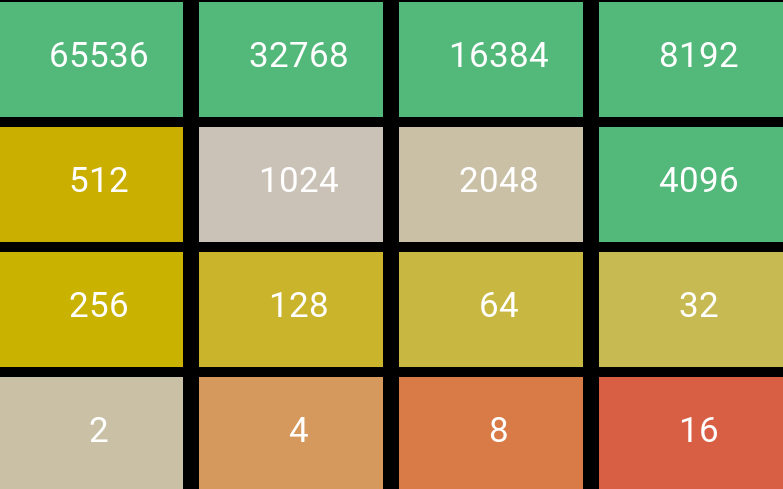
\includegraphics[width=0.5\linewidth]{perfect_monotonic}
\end{figure}
$R\low{mono}(s)$ is computed by following algorithm:
\begin{program}
\BEGIN \\ %
reward = 0\rcomment{\footnotesize Reward initally zero}

\FOR rows\ |in|\ board \DO \rcomment{\footnotesize Iterating over all four rows}
\Delta row = |elementwise\_differences|(row) \rcomment{\footnotesize Array of elementwise differences for the row}
\IF |idx|(row)\ \%\ 2 = 0\ \rcomment{\footnotesize If the row is uneven}
\IF |all|(\Delta row) > 0\ \DO 
reward 	\mathrel{{+}{+}} \OD\END|if| \rcomment{\footnotesize If the entire row is ascending, +1 to reward}
\ELSE \rcomment{\footnotesize If the row/column is even}
 	\IF |all|(\Delta row) < 0\ \DO 
reward 	\mathrel{{+}{+}} \OD\END|if| \rcomment{\footnotesize If the entire row/column is \textit{descending}, +1 to reward}
\OD\END|if|
reward = \frac{reward}{4} \rcomment{\footnotesize Reward is standardized to interval 0, 1}
\END 
\end{program}
\item \textit{Empty tiles} The number of empty tiles on the board is counted and divided by the maximum possible amount, 14, such that the starting position $s_1$ rewards +1
\item \textit{Merges} The sum of combined number of possible tile merges for all four possible actions divided by the maximum number, 32.
\item \textit{Highest tile in corner} Returns +1 if the maximum tile on the board is in one of the four corners.
\end{itemize}
The combined heuristic reward function used was
\begin{equation}\label{key}
R\low{heur}(s) = 3 \cdot R\low{mono}(s) + R\low{empty}(s) + R\low{merge}(s) + 3 \cdot  R\low{high}(s)
\end{equation}
to favour the effective strategies of monotonicity and always keeping the highest tile in the corner.
\subsection{Pseudo Code: Learning Process}\label{pseudo}
\begin{program}
	\BEGIN \\ %
	\mbox{|Initialize| $\pi$} \rcomment{\footnotesize Policy network initialized randomly}
	\FOR i= 1 \TO 500 \DO \rcomment{\footnotesize Play 500 batches}
	\FOR j= 1 \TO 50 \DO \rcomment{\footnotesize Each batch is 50 games}
	s = s_1 \rcomment{\footnotesize Game state $s$ is reset to first state}
	\WHILE game \neq over \DO
	p = \pi(s) \rcomment{\footnotesize Probabilities of actions computed by feed forward}
	a = |sample|(p) \rcomment{\footnotesize The chosen action randomly sampled from multinomial prob.}
	s = s(a) \rcomment{\footnotesize Action is taken}
	r = R(s) \rcomment{\footnotesize Reward function computes reward of game sate}
	|append|\ a \TO actions_j
	|append|\ r \TO rewards_j\OD \rcomment{\footnotesize Action and reward of each turn saved}
	
	r_j = |discount|(|standardize|(rewards_j), \ \gamma = 0.95)\OD
	\rcomment{\footnotesize Discounted sum of rewards for each game computed}
	\nabla \pi = |backpropagate|(\pi,\ r_{j..50},\ actions_{j..50})
	\rcomment{\footnotesize Gradient of $\pi$ computed using rewards as gradients for the sampled output neurons} 
	\pi = |optimize|(\pi,\ \nabla \pi,\ \alpha = 0.001)\OD  
	\rcomment{\footnotesize Optimizer changes parameters for policy network with regards to learning rate}
	\END
\end{program}


\subsection{Distributions of Max Tiles of All Agents}\label{mtile}

\begin{table}[H]
	\centering
	\begin{tabular}{@{}l|llll@{}}
		\toprule
		Layers / Reward& Score & Variance & Heuristics & Combination\\ \midrule
		256, 16, 4     &   \shortstack[l]{16: 0.03\pro\\32: 1.08\pro\\64: 11.9\pro\\128: 42.6\pro\\256: 40.1\pro\\512: 4.24\pro\\1024: 0.01\pro}     &    \shortstack[l]{16: 0.04\pro\\32: 1.31\pro\\64: 11.8\pro\\128: 44.2\pro\\256: 40.2\pro\\512: 2.41\pro\\ \ \\ \ \\ \ \\ \ }       &            \shortstack[l]{16: 0.08\pro\\32: 1.95\pro\\64: 14.7\pro\\128: 45.7\pro\\256: 33.6\pro\\512: 3.99\pro\\1024: 0.01\pro} &                                             \shortstack[l]{16: 0.04\pro\\32: 1.39\pro\\64: 14.8\pro\\128: 43.9\pro\\256: 35.5\pro\\512: 4.39\pro\\1024: 0.02\pro}             \\\\
		256, 100, 50, 4 & \shortstack[l]{16: 0.05\pro\\32: 1.14\pro\\64: 12.9\pro\\128: 43.1\pro\\256: 38.8\pro\\512: 3.95\pro\\ \ \\ \ \\ \ \\ \ }       &  \shortstack[l]{8: 0.14\pro\\16: 1.74\pro\\32: 7.94\pro\\64: 26.9\pro\\128: 43.2\pro\\256: 19.5\pro\\512: 0.53\pro\\ \ \\ \ \\ \ \\ \ }         &   \shortstack[l]{16: 0.01\pro\\32: 1.05\pro\\64: 12.4\pro\\128: 43.0\pro\\256: 40.0\pro\\512: 3.51\pro\\ \ \\ \ \\ \ \\ \ }          & \shortstack[l]{16: 0.03\pro\\32: 0.95\pro\\64: 12.6\pro\\128: 41.3\pro\\256: 40.0\pro\\512: 5.11\pro\\1024: 0.02\pro}                                                                        \\ \bottomrule
	\end{tabular}
\end{table}
Random Agent:   8: 0.03\pro, 16: 0.30\pro, 32: 6.76\pro, 64: 37.7\pro, 128: 47.5\pro, 256: 7.71\pro

\subsection{Plots of Learning Processes of All Agents}\label{plotlearn}
\begin{figure}[H]
	\centering
	\includegraphics[width=\linewidth]{"train_score_simple"}
	\caption{Training of agent with simple policy network and score as reward}
\end{figure}
\begin{figure}[H]
	\centering
	\includegraphics[width=\linewidth]{"train_variance_simple"}
	\caption{Training of agent with simple policy network and variance as reward}
\end{figure}

\begin{figure}[H]
	\centering
	\includegraphics[width=\linewidth]{"train_heuristics_simple"}
	\caption{Training of agent with simple policy network and heuristics as reward}
\end{figure}

\begin{figure}[H]
	\centering
	\includegraphics[width=\linewidth]{"train_combination_simple"}
	\caption{Training of agent with simple policy network and combination of reward functions as reward}
\end{figure}


\begin{figure}[H]
	\centering
	\includegraphics[width=\linewidth]{"train_score_complex"}
	\caption{Training of agent with complex policy network and score as reward}
\end{figure}
\begin{figure}[H]
	\centering
	\includegraphics[width=\linewidth]{"train_variance_complex"}
	\caption{Training of agent with complex policy network and variance as reward}
\end{figure}

\begin{figure}[H]
	\centering
	\includegraphics[width=\linewidth]{"train_heuristics_complex"}
	\caption{Training of agent with complex policy network and heuristics as reward}
\end{figure}

\begin{figure}[H]
	\centering
	\includegraphics[width=\linewidth]{"train_combination_complex"}
	\caption{Training of agent with complex policy network and combination of reward functions as reward}
\end{figure}
\subsection{Histograms of Results}\label{hist}
Left plot is the scores of \textit{all} games, right plot is the mean scores of the 700 batches of size 50 which is the metric used for the confidence intervals.
\begin{figure}[H]
	\centering
	\includegraphics[width=\linewidth]{"eval_score_simple"}
	\caption{Evaluation of agent with simple policy network and score as reward}
\end{figure}
\begin{figure}[H]
	\centering
	\includegraphics[width=\linewidth]{"eval_variance_simple"}
	\caption{Evaluation of agent with simple policy network and variance as reward}
\end{figure}

\begin{figure}[H]
	\centering
	\includegraphics[width=\linewidth]{"eval_heuristics_simple"}
	\caption{Evaluation of agent with simple policy network and heuristics as reward}
\end{figure}

\begin{figure}[H]
	\centering
	\includegraphics[width=\linewidth]{"eval_combination_simple"}
	\caption{Evaluation of agent with simple policy network and combination of reward functions as reward}
\end{figure}


\begin{figure}[H]
	\centering
	\includegraphics[width=\linewidth]{"eval_score_complex"}
	\caption{Evaluation of agent with complex policy network and score as reward}
\end{figure}
\begin{figure}[H]
	\centering
	\includegraphics[width=\linewidth]{"eval_variance_complex"}
	\caption{Evaluation of agent with complex policy network and variance as reward}
\end{figure}

\begin{figure}[H]
	\centering
	\includegraphics[width=\linewidth]{"eval_heuristics_complex"}
	\caption{Evaluation of agent with complex policy network and heuristics as reward}
\end{figure}

\begin{figure}[H]
	\centering
	\includegraphics[width=\linewidth]{"eval_combination_complex"}
	\caption{Evaluation of agent with complex policy network and combination of reward functions as reward}
\end{figure}
\end{document}
